\usetikzlibrary{patterns}

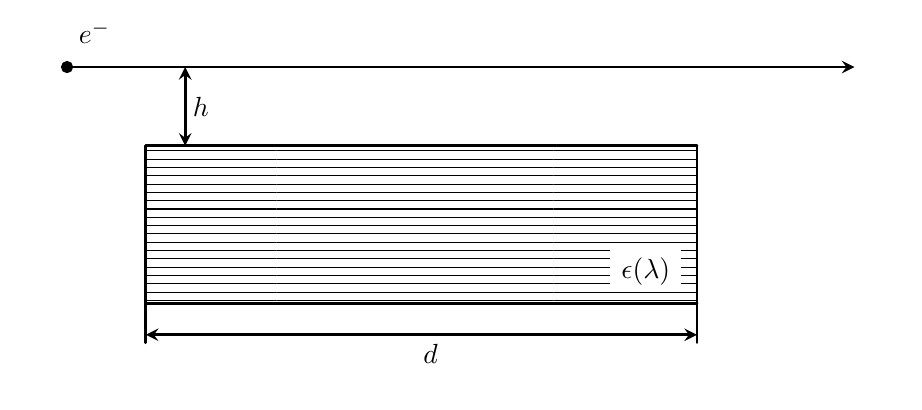
\begin{tikzpicture}[line cap=round,line join=round,>=stealth,x=1cm,y=1cm]

\clip(-0.5,-4) rectangle (10.5,0.5);

\fill[line width=1pt,fill=black,pattern=horizontal lines,pattern color=black] (1,-1) -- (8,-1) -- (8,-3) -- (1,-3) -- cycle;
\fill[line width=2pt,color=white,fill=white,fill opacity=1] (6.9,-2.3) -- (7.8,-2.3) -- (7.8,-2.8) -- (6.9,-2.8) -- cycle;

\draw [->,line width=1pt] (0,0) -- (10,0);
\draw [line width=1pt] (1,-1)-- (8,-1);
\draw [line width=1pt] (8,-1)-- (8,-3);
\draw [line width=1pt] (8,-3)-- (1,-3);
\draw [line width=1pt] (1,-3)-- (1,-1);
\draw [line width=1pt] (1,-3)-- (1,-3.5);
\draw [line width=1pt] (8,-3)-- (8,-3.5);

\draw [->,line width=1pt] (3.2,-3.4) -- (8,-3.4);
\draw [->,line width=1pt] (3.2,-3.4) -- (1,-3.4);
\draw (4.4,-3.4) node[anchor=north west] {$d$};

\draw [->,line width=1pt] (1.5,-0.5) -- (1.5,0);
\draw [->,line width=1pt] (1.5,-0.5) -- (1.5,-1);
\draw (1.7,-0.5) node[anchor=center] {$h$};

% \draw [line width=1pt,color=white] (7,-2.3)-- (7.8,-2.3);
% \draw [line width=1pt,color=white] (7.8,-2.3)-- (7.8,-2.8);
% \draw [line width=1pt,color=white] (7.8,-2.8)-- (7,-2.8);
% \draw [line width=1pt,color=white] (7,-2.8)-- (7,-2.3);
\draw (7.35,-2.6) node[anchor=center] {$\epsilon(\lambda)$};

\draw (0.025897872502580122,0.7) node[anchor=north west] {$e^-$};


\draw [fill=black] (0,0) circle (2pt);
\end{tikzpicture}